\chapter{الطبقات الإلكترونية والجدول الدوري}\label{ch:g10:electron-shells}

يتوهج النيون بلون أحمر برتقالي في اللافتات؛ والصوديوم، \omterm{def:g9:periodic-table-first-look:metal}{الفلز} اللين، يشتعل في
الماء؛ والكلور غاز أصفر مخضرّ خانق. ومع ذلك لا تختلف ذراتها إلا \omterm{def:g9:inside-the-atom:proton}{ببروتون} أو
اثنين: للنيون 10، وللصوديوم 11، وللكلور 17. فلماذا يختلف الجاران في \omterm{def:g9:periodic-table-first-look:periodic-table}{الجدول
الدوري} في سلوكهما إلى هذا الحد، بينما يتشابه الصوديوم والبوتاسيوم، المتباعدان
في \omterm{def:g9:inside-the-atom:atomic-number}{العدد الذري}، إلى هذا الحد؟ يكمن الجواب في طريقة ترتيب \omterm{def:g9:inside-the-atom:nucleus}{إلكترونات} \omterm{def:g7:atoms-and-molecules:atom}{الذرة}.

\begin{recall}
في \omterm{def:g9:inside-the-atom:nucleus}{نواة} \omterm{def:g7:atoms-and-molecules:atom}{الذرة} $Z$ بروتونًا، وحولها، إذا كانت متعادلة، $Z$ إلكترونًا
(\cref{ch:g9:inside-the-atom}). ويرتّب \omterm{def:g9:periodic-table-first-look:periodic-table}{الجدول الدوري} العناصر بحسب $Z$ في
دورات (صفوف) وزمر (أعمدة)؛ وعناصر \omterm{def:g9:periodic-table-first-look:period}{الزمرة} الواحدة تتشابه في سلوكها
(\cref{ch:g9:periodic-table-first-look}). وتكتسب \omterm{def:g7:atoms-and-molecules:atom}{الذرات} \omterm{def:g9:inside-the-atom:nucleus}{إلكترونات} أو تفقدها
فتصير \omterm{def:g9:ions:ion}{أيونات} (\cref{ch:g9:ions}).
\end{recall}

\section{التوزيع الإلكتروني}

\begin{definition}[الطبقات والطبقات الفرعية والتوزيع الإلكتروني]\label{def:g10:electron-shells:configuration}
تترتب \omterm{def:g9:inside-the-atom:nucleus}{إلكترونات} \omterm{def:g7:atoms-and-molecules:atom}{الذرة} في \emph{طبقات}\index{طبقة}، مرقّمة
$n = 1, 2, 3, \ldots$ من \omterm{def:g9:inside-the-atom:nucleus}{النواة} نحو الخارج؛ وكلما كبر $n$ ابتعدت
\omterm{def:g9:inside-the-atom:nucleus}{الإلكترونات} عن \omterm{def:g9:inside-the-atom:nucleus}{النواة} وضعف ارتباطها بها. وتنقسم كل طبقة إلى
\emph{طبقات فرعية}\index{طبقة فرعية} يُرمز إلى كل منها بحرف: للطبقة 1 طبقة
فرعية s، أي 1s، وللطبقة 2 طبقتان فرعيتان s وp، أي 2s و2p، وللطبقة 3 الطبقتان 3s
و3p (و3d، التي سنلقاها لاحقًا). والطبقة الفرعية s تتسع لإلكترونين على
الأكثر، والطبقة الفرعية p لستة. و\emph{التوزيع الإلكتروني}\index{توزيع إلكتروني}
\omterm{def:g7:atoms-and-molecules:atom}{لذرة} يذكر طبقاتها الفرعية المشغولة مع أعداد إلكتروناتها أُسسًا:
$1\mathrm{s}^2\,2\mathrm{s}^2\,2\mathrm{p}^4$ للأكسجين.
\end{definition}

\begin{method}[كتابة التوزيع الإلكتروني، حتى $Z = 20$]\label{met:g10:electron-shells:write}
\begin{enumerate}
  \item عُدّ \omterm{def:g9:inside-the-atom:nucleus}{الإلكترونات}: $Z$ \omterm{def:g7:atoms-and-molecules:atom}{للذرة} المتعادلة.
  \item املأ \omterm{def:g10:electron-shells:configuration}{الطبقات الفرعية} بهذا الترتيب، كل واحدة حتى حدها الأقصى قبل
        البدء في التالية:
        \[
          1\mathrm{s} \to 2\mathrm{s} \to 2\mathrm{p} \to 3\mathrm{s} \to
          3\mathrm{p} \to 4\mathrm{s}.
        \]
  \item تحقق من أن مجموع الأسس يساوي عدد \omterm{def:g9:inside-the-atom:nucleus}{الإلكترونات}.
\end{enumerate}
الصوديوم، $Z = 11$: $1\mathrm{s}^2\,2\mathrm{s}^2\,2\mathrm{p}^6\,3\mathrm{s}^1$.
الكلور، $Z = 17$: $1\mathrm{s}^2\,2\mathrm{s}^2\,2\mathrm{p}^6\,3\mathrm{s}^2\,3\mathrm{p}^5$.
الكالسيوم، $Z = 20$: $1\mathrm{s}^2\,2\mathrm{s}^2\,2\mathrm{p}^6\,3\mathrm{s}^2\,3\mathrm{p}^6\,4\mathrm{s}^2$.
\end{method}

\begin{omfigure}
\begin{tikzpicture}[font=\small, y=0.95cm]
  \draw[->, black!60] (-0.4,0) -- (-0.4,5.4) node[above, align=center, font=\footnotesize]
    {أبعد عن\\ النواة};
  \foreach \y/\lab/\n/\x in {0.3/1s/2/0.5, 1.3/2s/2/0.5, 1.9/2p/6/2.4, 3.0/3s/2/0.5,
      3.6/3p/6/2.4, 4.4/4s/2/0.5} {
    \foreach \k in {1,...,\n} \draw[omDef, fill=omDef!10] (\x+0.42*\k-0.42,\y) rectangle ++(0.36,0.36);
    \node[anchor=east] at (\x-0.05,\y+0.18) {\lab};
  }
  \node[anchor=west, font=\footnotesize] at (5.3,0.48) {\foreignlanguage{arabic}{الطبقة \babelsublr{1}: إلكترونان على الأكثر}};
  \node[anchor=west, font=\footnotesize] at (5.3,1.7) {\foreignlanguage{arabic}{الطبقة \babelsublr{2}: $2 + 6 = 8$}};
  \node[anchor=west, font=\footnotesize] at (5.3,3.4) {\foreignlanguage{arabic}{الطبقة \babelsublr{3}: $2 + 6 = 8$ (حتى $Z = 18$)}};
  \node[anchor=west, font=\footnotesize] at (5.3,4.58) {\foreignlanguage{arabic}{تمتلئ \babelsublr{4s} قبل \babelsublr{3d}}};
\end{tikzpicture}

{\small ترتيب الملء حتى $Z = 20$. كل مربع صغير مكان \omterm{def:g9:inside-the-atom:nucleus}{لإلكترون} واحد: \omterm{def:g10:electron-shells:configuration}{للطبقة
الفرعية} s مكانان، وللطبقة الفرعية p ستة.}
\end{omfigure}

\section{إلكترونات التكافؤ}

\begin{definition}[إلكترونات التكافؤ والإلكترونات الداخلية]\label{def:g10:electron-shells:valence}
\omterm{def:g9:inside-the-atom:nucleus}{إلكترونات} \omterm{def:g10:electron-shells:configuration}{الطبقة} الخارجية المشغولة (\omterm{def:g10:electron-shells:configuration}{الطبقة} ذات أكبر $n$) هي
\emph{إلكترونات التكافؤ}\index{إلكترون تكافؤ}؛ والأخرى هي
\emph{الإلكترونات الداخلية}\index{إلكترون داخلي}. ولا يشارك في التفاعلات
الكيميائية إلا \omterm{def:g9:inside-the-atom:nucleus}{إلكترونات} التكافؤ.
\end{definition}

\begin{example}[عدّ إلكترونات التكافؤ]\label{ex:g10:electron-shells:count}
الأكسجين، $1\mathrm{s}^2\,2\mathrm{s}^2\,2\mathrm{p}^4$: \omterm{def:g10:electron-shells:configuration}{الطبقة} الخارجية $n =
2$، فله $2 + 4 = 6$ \omterm{def:g9:inside-the-atom:nucleus}{إلكترونات} تكافؤ. الصوديوم، $\ldots 3\mathrm{s}^1$:
\omterm{def:g10:electron-shells:valence}{إلكترون تكافؤ} واحد. الكلور، $\ldots 3\mathrm{s}^2\,3\mathrm{p}^5$: 7.
النيون، $1\mathrm{s}^2\,2\mathrm{s}^2\,2\mathrm{p}^6$: 8، أي \omterm{def:g10:electron-shells:configuration}{طبقة} ممتلئة.
\end{example}

\section{إعادة بناء الجدول من التوزيعات الإلكترونية}

\begin{proposition}[الدورة والزمرة من التوزيع الإلكتروني]\label{prop:g10:electron-shells:table}
للعناصر حتى $Z = 20$:
\begin{itemize}
  \item \omterm{def:g9:periodic-table-first-look:period}{دورة} العنصر هي رقم طبقته الخارجية $n$؛
  \item لعناصر \omterm{def:g9:periodic-table-first-look:period}{الزمرة} الواحدة العدد نفسه من \omterm{def:g10:electron-shells:valence}{إلكترونات التكافؤ} ---
        واحد في \omterm{def:g9:periodic-table-first-look:period}{الزمرة} 1، واثنان في \omterm{def:g9:periodic-table-first-look:period}{الزمرة} 2، ومن ثلاثة إلى ثمانية في
        الزمر من 13 إلى 18 (والهيليوم، بإلكترونيه، استثناء).
\end{itemize}
ويكوّن العمودان الأيسران، حيث تدخل \omterm{def:g9:inside-the-atom:nucleus}{الإلكترونات} الأخيرة \omterm{def:g10:electron-shells:configuration}{طبقة فرعية} s، الفئة
s؛ وتكوّن الزمر من 13 إلى 18 الفئة p.
\end{proposition}

\begin{omfigure}
\omperiodictable[upto=20, f block=false, cell=0.86cm, colour=blocks, legend=true,
  values={H/1,He/2,Li/2.1,Be/2.2,B/2.3,C/2.4,N/2.5,O/2.6,F/2.7,Ne/2.8,
    Na/2.8.1,Mg/2.8.2,Al/2.8.3,Si/2.8.4,P/2.8.5,S/2.8.6,Cl/2.8.7,Ar/2.8.8,
    K/2.8.8.1,Ca/2.8.8.2}]

{\small العناصر العشرون الأولى، مع عدد \omterm{def:g9:inside-the-atom:nucleus}{الإلكترونات} في كل \omterm{def:g10:electron-shells:configuration}{طبقة} تحت الرمز
($2.8.1$ للصوديوم: 2 في \omterm{def:g10:electron-shells:configuration}{الطبقة} 1، و8 في \omterm{def:g10:electron-shells:configuration}{الطبقة} 2، و1 في \omterm{def:g10:electron-shells:configuration}{الطبقة} 3).
وتميّز الألوان الفئتين s وp.}
\end{omfigure}

\section{العائلات}

\begin{definition}[العائلات الكيميائية]\label{def:g10:electron-shells:family}
\emph{العائلة الكيميائية}\index{عائلة كيميائية} \omterm{def:g9:periodic-table-first-look:period}{زمرة} من \omterm{def:g9:periodic-table-first-look:periodic-table}{الجدول الدوري}
تشترك عناصرها في خصائصها الكيميائية الرئيسية. وثلاث عائلات لها أسماء:
\emph{الفلزات القلوية}\index{فلز قلوي} (\omterm{def:g9:periodic-table-first-look:period}{الزمرة} 1 ما عدا الهيدروجين:
الليثيوم، والصوديوم، والبوتاسيوم\dots)، وهي \omterm{def:g9:periodic-table-first-look:metal}{فلزات} لينة تتفاعل بشدة مع الماء؛
و\emph{الهالوجينات}\index{هالوجين} (\omterm{def:g9:periodic-table-first-look:period}{الزمرة} 17: الفلور، والكلور، والبروم،
واليود)، وهي لافلزات ملونة نشيطة؛ و\emph{الغازات النبيلة}\index{غاز نبيل}
(\omterm{def:g9:periodic-table-first-look:period}{الزمرة} 18: الهيليوم، والنيون، والأرغون\dots)، وهي لا تكاد تتفاعل مع أي
شيء.
\end{definition}

\begin{proposition}[لماذا تتشابه العائلة في سلوكها]\label{prop:g10:electron-shells:why}
لعناصر العائلة الواحدة العدد نفسه من \omterm{def:g10:electron-shells:valence}{إلكترونات التكافؤ}، والكيمياء شأن
\omterm{def:g10:electron-shells:valence}{إلكترونات التكافؤ}: فلليثيوم والصوديوم والبوتاسيوم كلها \omterm{def:g9:inside-the-atom:nucleus}{إلكترون} واحد،
وللهالوجينات سبعة، وللغازات النبيلة \omterm{def:g10:electron-shells:configuration}{طبقة} خارجية
ممتلئة.
\end{proposition}

\begin{omfigure}
\omperiodictable[colour=families, legend=true, cell=0.86cm, f block=false]

{\small عائلات \omterm{def:g9:periodic-table-first-look:periodic-table}{الجدول الدوري}: \omterm{def:g10:electron-shells:family}{الفلزات القلوية}، \omterm{def:g10:electron-shells:family}{والفلزات القلوية} الترابية
(\omterm{def:g9:periodic-table-first-look:period}{الزمرة} 2)، \omterm{def:g10:electron-shells:family}{والهالوجينات}، \omterm{def:g10:electron-shells:family}{والغازات النبيلة}.}
\end{omfigure}

\begin{omfigure}
\begin{minipage}[b]{0.48\linewidth}\centering
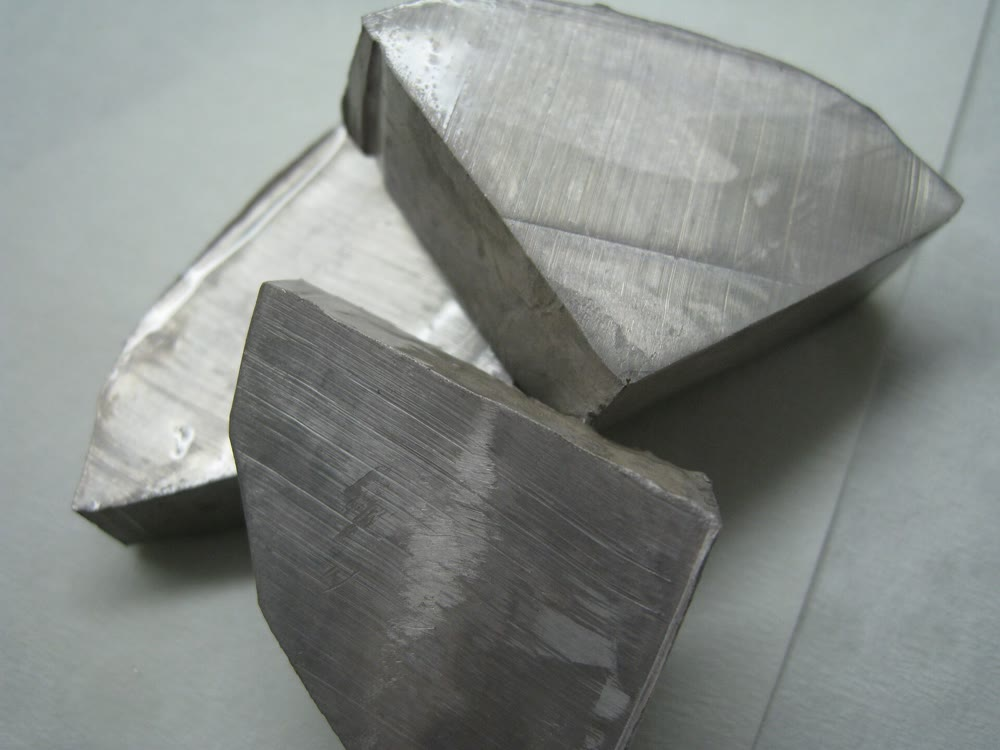
\includegraphics[width=\linewidth,height=4.4cm,keepaspectratio]{images/book1/sodium.jpg}

{\small الصوديوم، \omterm{def:g10:electron-shells:family}{فلز قلوي}، مقطوعًا بسكين: لين وفضي حين يُقطع حديثًا، ويبهت
فورًا في \omterm{def:g4:air-a-mixture-of-gases:air}{الهواء}. تصوير: Dnn87، CC BY-SA 3.0.}
\end{minipage}\hfill
\begin{minipage}[b]{0.48\linewidth}\centering
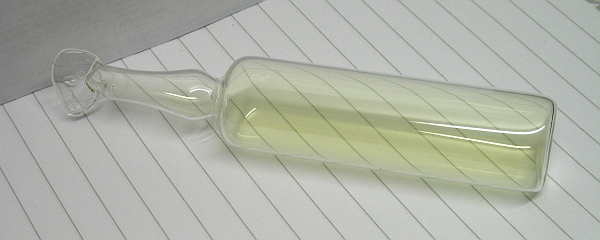
\includegraphics[width=\linewidth,height=4.4cm,keepaspectratio]{images/book1/chlorine-ampoule.jpg}

{\small الكلور، \omterm{def:g10:electron-shells:family}{هالوجين}: غاز أصفر مخضرّ، محفوظ هنا في أمبولة
زجاجية. تصوير: ف.~أولن، CC BY-SA 3.0.}
\end{minipage}
\end{omfigure}

\begin{inthelab}[الصوديوم في الماء]
خلف حاجز واقٍ يُسقط المعلم قطعة من الصوديوم بحجم حبة الأرز في وعاء كبير من
الماء. فتطفو، وتنصهر فتصير كرة لامعة، وتجري هنا وهناك فائرة حتى تختفي؛
والغاز المنطلق هو الهيدروجين، والماء الباقي قاعدي.
\end{inthelab}

\begin{safety}{\ghs[0.75cm]{GHS02}\ghs[0.75cm]{GHS05}\quad\ghs[0.75cm]{GHS03}\ghs[0.75cm]{GHS06}}
% ledger: ghs:Na, ghs:Cl2
الصوديوم: يطلق مع الماء هيدروجينًا قابلًا للاشتعال (GHS02)، ويسبب حروقًا
شديدة (GHS05). الكلور: غاز مؤكسد (GHS03)، سام إذا استُنشق (GHS06)، وهو
أيضًا مهيّج وشديد السمية للأحياء المائية. ولا يتناولهما إلا
المعلم.
\end{safety}

\section{الأيونات المستقرة وقاعدة الغاز النبيل}

\begin{definition}[قاعدتا الثنائية والثمانية]\label{def:g10:electron-shells:octet}
\omterm{def:g10:electron-shells:family}{الغازات النبيلة}، بطبقتها الخارجية الممتلئة، لا تكاد تتفاعل: فتوزيعها
الإلكتروني مستقر على نحو خاص. وحين تكوّن \omterm{def:g7:atoms-and-molecules:atom}{ذرات} العناصر الأولى \omterm{def:g9:ions:ion}{أيونات} فإنها
تكتسب \omterm{def:g9:inside-the-atom:nucleus}{إلكترونات} أو تفقدها لتبلغ \omterm{def:g10:electron-shells:configuration}{التوزيع الإلكتروني} لأقرب \omterm{def:g10:electron-shells:family}{غاز نبيل}: إلكترونين
في \omterm{def:g10:electron-shells:configuration}{الطبقة} 1، مثل الهيليوم، لأخف \omterm{def:g7:atoms-and-molecules:atom}{الذرات} --- وهي
\emph{قاعدة الثنائية}\index{قاعدة الثنائية} --- وثمانية \omterm{def:g9:inside-the-atom:nucleus}{إلكترونات} في \omterm{def:g10:electron-shells:configuration}{الطبقة}
الخارجية، مثل النيون أو الأرغون، \omterm{def:g7:atoms-and-molecules:atom}{للذرات} الأخرى --- وهي
\emph{قاعدة الثمانية}\index{قاعدة الثمانية}.
\end{definition}

\begin{example}[أيونات تتنبأ بها القاعدة]\label{ex:g10:electron-shells:ions}
الصوديوم، $2.8.1$، يفقد \omterm{def:g9:inside-the-atom:nucleus}{إلكترون} تكافئه الوحيد: \ce{Na+}، $2.8$، مثل
النيون. والمغنيسيوم، $2.8.2$، يفقد اثنين: \ce{Mg^{2+}}. والألومنيوم، $2.8.3$،
يفقد ثلاثة: \ce{Al^{3+}}. والكلور، $2.8.7$، يكتسب واحدًا: \ce{Cl-}، $2.8.8$،
مثل الأرغون. والأكسجين، $2.6$، يكتسب اثنين: \ce{O^{2-}}. والكبريت، $2.8.6$:
\ce{S^{2-}}. والليثيوم، $2.1$، يفقد واحدًا فيبقى له $2$، مثل الهيليوم:
\ce{Li+}.
\end{example}

\begin{omfigure}
\begin{tikzpicture}[font=\small]
  \foreach \x/\nm/\cfg/\col in {0/{Na}/{$1\mathrm{s}^2\,2\mathrm{s}^2\,2\mathrm{p}^6\,3\mathrm{s}^1$}/omDef,
      5.8/{\ce{Na+}}/{$1\mathrm{s}^2\,2\mathrm{s}^2\,2\mathrm{p}^6$}/omProp,
      11.0/{Ne}/{$1\mathrm{s}^2\,2\mathrm{s}^2\,2\mathrm{p}^6$}/gray} {
    \node[draw=\col, fill=\col!6, rounded corners=2pt, align=center, text width=3.4cm]
      at (\x,0) {\textbf{\nm}\\ \cfg};
  }
  \draw[->, thick, omProp] (2.0,0) -- (3.8,0) node[midway, above, font=\footnotesize] {\foreignlanguage{arabic}{يفقد \babelsublr{1} \ce{e-}}};
  \node at (8.4,0) {$=$};
  \node[font=\footnotesize, align=center] at (8.4,-0.75) {التوزيع\\ نفسه};
\end{tikzpicture}

{\small \omterm{def:g9:ions:ion}{لأيون} الصوديوم \omterm{def:g10:electron-shells:configuration}{التوزيع الإلكتروني} للنيون، أقرب \omterm{def:g10:electron-shells:family}{غاز
نبيل}.}
\end{omfigure}

\begin{remark}[حدود القاعدة]\label{rem:g10:electron-shells:limits}
تصلح القاعدة جيدًا للعناصر العشرين الأولى وأيوناتها البسيطة. لكن عناصر كثيرة،
مثل الحديد (\ce{Fe^{2+}} و\ce{Fe^{3+}})، لا تتبعها؛ والأسباب، ووصف أدق
\omterm{def:g9:inside-the-atom:nucleus}{للإلكترونات}، تأتي في كتاب السنة الجامعية الأولى.
\end{remark}

\section{تمارين}

\begin{exercise}[$\star$]\label{exo:g10:electron-shells:1}
اكتب التوزيعات الإلكترونية للكربون ($Z = 6$)، والنيتروجين ($Z = 7$)،
والمغنيسيوم ($Z = 12$).
\end{exercise}

\begin{exercise}[$\star$]\label{exo:g10:electron-shells:2}
كم \omterm{def:g10:electron-shells:valence}{إلكترون تكافؤ} للكربون والنيتروجين والمغنيسيوم؟
\end{exercise}

\begin{exercise}[$\star$]\label{exo:g10:electron-shells:3}
في أي \omterm{def:g9:periodic-table-first-look:period}{دورة} وأي \omterm{def:g9:periodic-table-first-look:period}{زمرة} يقع العنصر ذو \omterm{def:g10:electron-shells:configuration}{التوزيع الإلكتروني}
$1\mathrm{s}^2\,2\mathrm{s}^2\,2\mathrm{p}^6\,3\mathrm{s}^2\,3\mathrm{p}^3$؟
\end{exercise}

\begin{exercise}[$\star$]\label{exo:g10:electron-shells:4}
سمِّ العائلات الثلاث في هذا الفصل وأعطِ عنصرين من كل منها.
\end{exercise}

\begin{exercise}[$\star$]\label{exo:g10:electron-shells:5}
اذكر \omterm{def:g10:electron-shells:octet}{قاعدة الثمانية}.
\end{exercise}

\begin{exercise}[$\star\star$]\label{exo:g10:electron-shells:6}
مستعينًا بقاعدة \omterm{def:g10:electron-shells:family}{الغاز النبيل}، أعطِ \omterm{def:g9:ions:ion}{الأيون} الذي يكوّنه البوتاسيوم ($Z = 19$)
والفلور ($Z = 9$)، مع توزيعيهما الإلكترونيين.
\end{exercise}

\begin{exercise}[$\star\star$]\label{exo:g10:electron-shells:7}
في \omterm{def:g10:electron-shells:configuration}{الطبقة} الثالثة لعنصر إلكترونان، وطبقته الثالثة هي طبقته الخارجية. أعطِ
توزيعه الإلكتروني وعدده الذري واسمه.
\end{exercise}

\begin{exercise}[$\star\star$]\label{exo:g10:electron-shells:8}
مستعينًا \omterm{def:g9:ions:ion}{بالأيونات} المستقرة، اكتب صيغة \omterm{def:g9:ions:ionic-compound}{المركب الأيوني} الذي يكوّنه المغنيسيوم
والكلور، ثم الألومنيوم والأكسجين.
\end{exercise}

\begin{exercise}[$\star\star$]\label{exo:g10:electron-shells:9}
انظر إلى جدول العناصر العشرين الأولى. أي العناصر لها العدد نفسه من \omterm{def:g10:electron-shells:valence}{إلكترونات
التكافؤ} الذي للأكسجين؟
\end{exercise}

\begin{exercise}[$\star\star$]\label{exo:g10:electron-shells:10}
لماذا لا يكوّن النيون، خلافًا للصوديوم والكلور، \omterm{def:g9:ions:ion}{أيونات} في التفاعلات
الكيميائية؟
\end{exercise}

\begin{exercise}[$\star\star$]\label{exo:g10:electron-shells:11}
\omterm{def:g9:ions:ion}{للأيون} \ce{X^{2+}} \omterm{def:g10:electron-shells:configuration}{التوزيع الإلكتروني} للأرغون. جد $X$.
\end{exercise}

\begin{exercise}[$\star\star\star$]\label{exo:g10:electron-shells:12}
للهيليوم إلكترونا تكافؤ لكنه يقع في \omterm{def:g9:periodic-table-first-look:period}{الزمرة} 18 لا في \omterm{def:g9:periodic-table-first-look:period}{الزمرة} 2. علّل بتوزيعه
الإلكتروني.
\end{exercise}

\begin{exercise}[$\star\star\star$]\label{exo:g10:electron-shells:13}
يتفاعل البوتاسيوم مع الماء بعنف أشد من الصوديوم. مستعينًا ببعد \omterm{def:g10:electron-shells:valence}{إلكترون التكافؤ}
عن \omterm{def:g9:inside-the-atom:nucleus}{النواة}، اقترح سببًا لذلك.
\end{exercise}

\begin{exercise}[$\star\star\star$]\label{exo:g10:electron-shells:14}
أعطِ التوزيعات الإلكترونية \omterm{def:g9:ions:ion}{للأيونات} \ce{S^{2-}} و\ce{Cl-} و\ce{K+}
و\ce{Ca^{2+}}. ما الذي تشترك فيه؟
\end{exercise}

\begin{exercise}[$\star\star\star$]\label{exo:g10:electron-shells:15}
عنصر من \omterm{def:g9:periodic-table-first-look:period}{الدورة} 3 يكوّن \omterm{def:g9:ions:ion}{الأيون} \ce{Y^{3-}}. جد زمرته وتوزيعه الإلكتروني
واسمه.
\end{exercise}

\section{مسألة: الياقوت الأحمر والياقوت الأزرق والكوراندوم}

\begin{problem}[{مسألة نهاية الأسبوع --- الإلكترونات وراء حجر كريم: من توزيعين
إلكترونيين إلى عدد الإلكترونات المنقولة في غرام واحد}]
\label{pb:g10:electron-shells:1}
الياقوت الأحمر والياقوت الأزرق صورتان كريمتان للكوراندوم، وهو \omterm{def:g9:ions:ionic-compound}{مركب أيوني} من
الألومنيوم والأكسجين؛ وأثر من \omterm{def:g9:periodic-table-first-look:metal}{فلزات} أخرى يعطيهما لونيهما. والكوراندوم صلب إلى
حد أنه يخدش كل شيء تقريبًا، ومسحوقه يُستعمل لصقل العدسات. خذ كتلة \omterm{def:g9:inside-the-atom:proton}{النوكليون}
\qty{1.67e-27}{kg}؛ \omterm{def:g7:atoms-and-molecules:atom}{وذرة} الألومنيوم 27 فيها 27 نوكليونًا، \omterm{def:g7:atoms-and-molecules:atom}{وذرة} الأكسجين 16 فيها 16.

\medskip
\noindent\textbf{الجزء الأول --- \omterm{def:g7:atoms-and-molecules:atom}{الذرات}.}
\begin{enumerate}
  \item أعطِ عدد \omterm{def:g9:inside-the-atom:proton}{البروتونات} \omterm{def:g9:inside-the-atom:nucleus}{والإلكترونات} في \omterm{def:g7:atoms-and-molecules:atom}{ذرة} الألومنيوم
        ($Z = 13$) وفي \omterm{def:g7:atoms-and-molecules:atom}{ذرة} الأكسجين ($Z = 8$).
  \item اكتب توزيعيهما الإلكترونيين.
  \item كم \omterm{def:g10:electron-shells:valence}{إلكترون تكافؤ} لكل منهما؟ وفي أي \omterm{def:g9:periodic-table-first-look:period}{دورة} وأي \omterm{def:g9:periodic-table-first-look:period}{زمرة}
        يقع كل منهما؟
  \item هل الألومنيوم \omterm{def:g9:periodic-table-first-look:metal}{فلز} أم \omterm{def:g9:periodic-table-first-look:metal}{لافلز}؟ والأكسجين؟
\end{enumerate}

\medskip
\noindent\textbf{الجزء الثاني --- \omterm{def:g9:ions:ion}{الأيونات}.}
\begin{enumerate}[resume]
  \item مستعينًا \omterm{def:g10:electron-shells:octet}{بقاعدة الثمانية}، أي \omterm{def:g9:ions:ion}{أيون} يكوّنه الألومنيوم؟ اكتب
        توزيعه الإلكتروني.
  \item أي \omterm{def:g9:ions:ion}{أيون} يكوّنه الأكسجين؟ اكتب توزيعه الإلكتروني.
  \item أي \omterm{def:g10:electron-shells:family}{غاز نبيل} له \omterm{def:g10:electron-shells:configuration}{التوزيع الإلكتروني} نفسه الذي للأيونين؟
  \item كم إلكترونًا تفقد \omterm{def:g7:atoms-and-molecules:atom}{ذرة} الألومنيوم، وكم إلكترونًا تكتسب \omterm{def:g7:atoms-and-molecules:atom}{ذرة}
        الأكسجين؟
\end{enumerate}

\medskip
\noindent\textbf{الجزء الثالث --- الصيغة.}
\begin{enumerate}[resume]
  \item جد صيغة الكوراندوم، المركب المتعادل المكوّن من هذين الأيونين.
  \item في وحدة صيغة واحدة، كم إلكترونًا تفقد \omterm{def:g7:atoms-and-molecules:atom}{ذرات} الألومنيوم؟ وكم تكتسب
        \omterm{def:g7:atoms-and-molecules:atom}{ذرات} الأكسجين؟
  \item لماذا يجب أن يتساوى هذان العددان؟
  \item يحوي الياقوت الأحمر أثرًا من \omterm{def:g9:ions:ion}{أيونات} الكروم \ce{Cr^{3+}} مكان
        بعض \omterm{def:g9:ions:ion}{أيونات} \ce{Al^{3+}}. لماذا يستطيع \omterm{def:g9:ions:ion}{أيون} \ce{Cr^{3+}} أن يحل محل
        \omterm{def:g9:ions:ion}{أيون} \ce{Al^{3+}} دون أن يُخل بالشحنات؟
\end{enumerate}

\medskip
\noindent\textbf{الجزء الرابع --- غرام واحد من الكوراندوم.}
\begin{enumerate}[resume]
  \item كم نوكليونًا في وحدة صيغة واحدة من الكوراندوم؟
  \item احسب كتلة وحدة صيغة واحدة (مع إهمال \omterm{def:g9:inside-the-atom:nucleus}{الإلكترونات}).
  \item كم وحدة صيغة في \qty{1}{g} من الكوراندوم؟
  \item كم \omterm{def:g9:ions:ion}{أيون} \ce{Al^{3+}} وكم \omterm{def:g9:ions:ion}{أيون} \ce{O^{2-}} يمثل ذلك؟
  \item لماذا يجوز إهمال \omterm{def:g9:inside-the-atom:nucleus}{الإلكترونات} في السؤال 14؟
  \item كم إلكترونًا انتقل من الألومنيوم إلى الأكسجين لصنع \qty{1}{g} من
        الكوراندوم؟
\end{enumerate}
\end{problem}
